 \section{Probabilidad condicional}
{}
Sean $A,B$ dos eventos tales que $P(A)>0.$
\begin{figure}
	\centering
	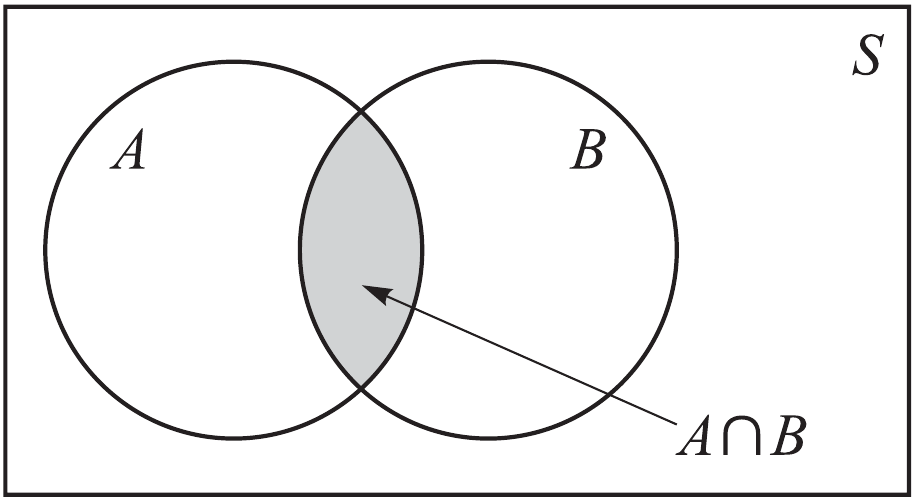
\includegraphics[width=5cm,keepaspectratio=true]{./pe/pands0103.png}
	% pands0103.png: 0x0 pixel, 300dpi, 0.00x0.00 cm, bb=
	\label{pands0103}
\end{figure}

Denotaremos por $P(B|A)$
la probabilidad de $B$ dado que $A$ haya ocurrido y diremos que es la \emph{probabilidad condicional} de $B$ dado $A.$


\begin{defn}[Probabilidad condicional]
	\begin{align}
		P(B|A)&=\dfrac{P(A\cap B)}{P(A)} \\
		P(A\cap B) &= P(A)P(B|A)
	\end{align}
\end{defn}


{}
\begin{rem}
	La probabilidad condicional satisface todos los axiomas de una función de probabilidad.  Podemos pensar $P(\cdot|A)$ como la función de probabilidad que se obtiene al reemplazar el espacio muestral $S$ por $A.$
\end{rem}


{}
\begin{ejemplo}
	\label{exmp:1.13}
	Encontrar la probabilidad de que una solo lanzamiento de un dado resulte en un número menor que $4$ si
	\begin{enumerate}
		\item no hay más información; 
		\item se sabe que el lanzamiento resultó en un número impar.
	\end{enumerate}
	
\end{ejemplo}


\subsection{Teoremas sobre Probabilidad Condicional}
{}
\begin{thm}
	\label{thm:1.9}
	Para cualesquiera tres eventos $A_{1},A_{2},A_{3},$ tenemos que
	\begin{align}
		\label{1.19}
		P(A_{1} \cap A_{2} \cap A_{3})=P(A_{1})P(A_{2}|A_{1})P(A_{3}|A_{1} \cap A_{2})
	\end{align}
\end{thm}


{}
\begin{thm}
	\label{thm:1.10} Si $S=A_{1}\sqcup ... \sqcup A_{N},$  entonces
	\begin{align}
		\label{1.20}
		P(A)=P(A_{1})P(A|A_{1})+...+P(A_{N})P(A|A_{N})
	\end{align}
\end{thm}


\subsection{Eventos independientes}
{}
Si $P(B|A)=P(B),$ i.e., la probabilidad de que $B$ ocurra no está afectada por la ocurrencia de $A,$ entonces diremos que $A$ y $B$ son independientes.


\begin{defn}
	$A$ y $B$ son eventos independientes si y solo si
	\begin{align}
		\label{1.21}
		P(A \cap B) = P(A)P(B).
	\end{align}
\end{defn}


{}
La definición se puede generalizar a más de dos eventos.  Por ejemplo, diremos que $A_{1},A_{2},A_{3}$ son eventos independientes si
\begin{align}
	k\neq j \rightarrow P(A_{j} \cap A_{k})=P(A_{j})P(A_{k}), \; j,k=1,2,3 
	\\ P(A_{1}\cap A_{2} \cap A_{3})=P(A_{1})P(A_{2})P(A_{3}).
\end{align}


{}
\begin{thm}[Teorema de Bayes]
	Si $S=A_{1}\sqcup A_{2} \sqcup...\sqcup A_{N},$ entonces
	\begin{align}
		\label{1.24}
		P(A_{k}|A) = \dfrac{P(A_{k})P(A|A_{k})}{\sum_{j} P(A_{j})P(A|A_{j})}
	\end{align}
	
\end{thm}




\begin{ejemplo}
	\label{solved:1.16}
	Demuestre el teorema de Bayes.
\end{ejemplo}



{}
\begin{ejemplo}
	\label{solved:1.15}
	La caja $I$ contiene 3 canicas rojas y 2 azules, mientras que la caja $II$ contiene $8$ canicas rojas y 8 azules. Una moneda se lanza: Si cae un sol, se escoge una moneda de la caja $I$ y si cae reverso, de la caja $II.$ Encuentre la probabilidad de obtener una canica roja.
\end{ejemplo}


{}
\begin{ejemplo}
	\label{solved:17}
	Supongamos que en el problema anterior, quien lanza la moneda no revela si ha caído reverso o sol (de manera que la caja de la que se obtiene la canica no se revela) pero revela que una canica roja se ha obtenido.?`Cual es la probabilidad de haber obtenido un sol?
\end{ejemplo}


